\documentclass[11pt, oneside]{article}   	% use "amsart" instead of "article" for AMSLaTeX format
\usepackage{geometry}                		% See geometry.pdf to learn the layout options. There are lots.
\geometry{letterpaper}                   		% ... or a4paper or a5paper or ... 
%\geometry{landscape}                		% Activate for for rotated page geometry
%\usepackage[parfill]{parskip}    		% Activate to begin paragraphs with an empty line rather than an indent
\usepackage{graphicx}				% Use pdf, png, jpg, or eps� with pdflatex; use eps in DVI mode
								% TeX will automatically convert eps --> pdf in pdflatex		
\usepackage{amssymb}
\usepackage{amsmath}
\usepackage{verbatim}

\title{Tweets, Tags, and \#Hashtags}
\author{Deirdre Quillen}
%\date{}							% Activate to display a given date or no date

\begin{document}
\maketitle
\section*{Introduction}
Part-of-speech tagging is a well-developed area of natural language processing. Building better part-of-speech taggers has been an ongoing competition among researchers in natural language processing since the 1980s.  Modern POS-taggers like the Stanford Tagger achieve over $97\%$ accuracy, and are constantly improving. Most of these POS-taggers tag traditional English text, such as one million words form the 1989 Wall Street Journal, which is a standard test for comparison between POS-taggers. 

As POS-taggers have had such success with traditional written texts (in English and other languages), it is a natural question whether these same techniques an be applied to more diverse media. This paper will optimize an averaged peceptron POS-tagger designed specifically for statuses on the website Twitter. There a several reasons a POS-tagger for Twitter might be interesting. Volumes of information pass through Twitter every day; the latest count is that there are $500$ million tweets sent on a typical day, with $5,700$ tweets per second \cite{twitterBlog}. Currently there are 200 million active users on Twitter every month \cite{gateTagger}. Twitter use particular explode during events such as the Super bowl, the 2011 Egyptian revolution, and major holidays. 

While POS-tagging has questionable usefulness in other natural language processing challenges such as parsing, \cite{bootstrap}, POS-taggers for Twitter have been attempted in natural language processing applications such as sentiment inference in this source \cite{sentiment}. However, a major block in the use of twitter POS-taggers is that they have not yet reached the level of POS-taggers for other texts. The author of \cite{sentiment} even cites this as a potential reason that POS-tags were not useful in the questions explored by this paper. Even the modern state of the art POS-tagger, the Stanford tagger, labels part of speech of words in tweets much less accurately than it does for other texts, even when trained on tweets. There are a couple reasons that POS-tagging for Twitter has not yet reached the same level of effectiveness of traditional part of speech tagging. Twitter statuses use much less standardized English than that that appears in the Wall Street journal. Twitter is a medium full of colloquialisms that can not even be categorized under traditional English parts of speech- for example, the colloquialism ``smh'' is short for the full phrase "shake my head". Spelling mistakes and typos create noise that learning algorithms have difficulty with, and lack of capitalization makes it harder for an algorithm to recognize proper nouns.

\section{Current Work}

Several recent papers have tackled the challenge of creating and improving POS-taggers for language on Twitter. In ``Part of Speech Tagging for Twitter: Annotation, Features, Experiments", a group of researchers from Carnegie Mellon University annotates a dataset of over $1,800$ tweets with their own labels and builds a POS-tagger based on a conditional random field. Their conditional random field uses features derived from Twitter orthography (spelling), tagging sequences, and phonetic normalization to handle spelling mistakes. They achieve approaching $90\%$ accuracy.

In ``Twitter Part-of-Speech Tagging for All: Overcoming Sparse and Noisy Data", a group of researchers makes adjustments to the state-of-the art Stanford tagger (which uses a maximum entropy dependency network) to improve its functionality on Twitter sentences. They make a comprehensive comparisons between the effectiveness of different taggers applied to Twitter. This paper, unlike the paper above, uses the traditional part-of-speech labels that are standard is research papers (the tags used in the paper above, and that I use, are broader). They improve the Stanford Tagger by creating a lookup list of common slang words, and by creating features to recognize and handle slang. Finally, they implement a "bootstrapping" method to train based on non-fully supervised data.

 In this paper I use an average perceptron model on the data set from ``Part of Speech Tagging for Twitter: Annotation, Features, Experiments". I use the exact tags that they define in their paper, and compare my results to those of the CRF.

\section{Averaged Perceptron}
A perceptron is very a simple machine learning model developed by Frank Rosenblatt at Cornell in 1957. A perceptron functions by finding a linear decision boundary in a dataset. While simple, a linear decision boundary cannot always be found, most famously in the XOR case. In the years since its invention, the limitations of perceptrons were discovered and published, and much of the research was abandoned for years. However, it remains that perceptrons are still one of the simplest and most effective tools in tagging for certain tasks. In 2002, Michael Collins achieved significant improvement int he current POS-tagging systems using an averaged perceptron model, and provided proof of convergence for the averaged perceptron algorithm for classification problems.\\

Variants of the averaged perceptron algorithms are still used in the some of the best modern part of speech taggers \cite{wikiPOS}. However, their most important advantage, particularly for this project, is their relative simplicity compared to CRF models. A competitive CRF models rely on dozens of complicated feature functions. The workings of an average perceptron model are much more simple.

\subsection{Basic Algorithm}
The basic broadly designed from a model of neurons in the brain. If we have an input vector $(x_1, x_2, \ldots, x_n)$ and a weight vector $(w_1, \ldots, w_n)$ we define our activation $a$ as the equation
\[ a = \left(\sum_{i=1}^n w_i x_i\right) + b\]
$b$ here is a constant that we call a bias. If $a$ is above a threshold $T$, then our "neuron" is fired. We can think of this as our model having assigned label $1$. If $a< T$, then our model has assigned label $0$. In this case we have a label set of two, $\{0, 1\}$.

\subsection{Features}
The above is the case for a model in which we have two label states. However, since our model has multiple labels, we predict labels in the following way. 

For a word $n_i$ at position $i$ in a sentence $S$, a set of features $F$ is created (F is some subset of the set of all features $F_{\text{total}}$). The features are based on all information up to position $i$: a feature might be, for example, the first letter of $n_i$, or the label of the previous word, $n_{i-1}$. To perform prediction, we assign an integer weight to each feature-label pair. So if we consider our word $n$ and its set of features $F$, we simply compute a score for each label by summing the weight for each feature. The predicted weight is the maximum score. Writing the weight as a function of a feature $f$ and a label $l$, the predicted label is
\[ \max_{l} \sum_{f \in F} w(f, l) \]
 We see these features behave much like an HMM or a CRF, in that the label of word $n_i$ is determined by the transition probability from previous labels in the sentence. \cite{bootstrap} Thus, we are able to essentially use the Viterbi algorithm for prediction.\\
 
The features I used in this model were those recommended by \cite{200words}:\\
\begin{tabular}{ l | c }
Feature & Description\\
\hline
$f_1 = b$ & Bias, a constant\\
$f_2 = n_i[-3:]$ & Suffix of word $n_i$, the last three letters.\\
$f_3 = n_i[1]$ & First letter of word $n_i$\\
$f_4 = l_{i-1}$ & The label of word $n_{i-1}$\\
$f_5 = l_{i-2}$ & The label of word $n_{i-2}$\\
$f_6 = (l_{i-1}, l_{i-2})$ & The pair of previous labels\\
$f_7 = n_i$ & The $i$th word $n_i$\\
$f_8 = (l_{i-1}, n_i)$ & The tag of the previous word and current word\\
$f_9 = n_{i-1}$ & The previous word\\
$f_{10} = n_{i-1}[-3:]$ & Suffix of word $n_{i-1}$\\
$f_{11} = n_{i-2}$ & The $(i-2)$th word\\
$f_{12} = n_{i+1}$ & The next word\\
$f_{13} = n_{i+1}[-3:]$ & Suffix of word $n_{i+1}$\\
$f_{14} = n_{i+2}$ & The $(i+2)$th word\\
\end{tabular}


\subsection{Training}
The training algorithm for a perceptron is very simple. Given a labelled dataset, the training algorithm loops through every word in the data set. For a given word, the above equation (which is essentially the Viterbi algorithm) predicts the label of the word. If this guess, is correct, the algorithm iterates to the next word. If not, the weight of the incorrect word is decreased by 1, and the weight of the correct word is increased by one. It is clear that if this algorithm were to loop over the same word sufficiently many times, it would correct to guess the correct label.

\subsection{Averaging}
A drawback of the perceptron algorithm is that if it runs to convergence, that it can overfit the given data \cite{200words}. For this reason, we take the average of all weights, and return this average to achieve optimal parameters. This average is taken over every possible instance of the weights: every time a weight is updated after an incorrect prediction, this new weight is accounted for in the average.

\subsection{Convergence}
While an averaged perceptron is guaranteed to converge \cite{collins}, it can be difficult to tune the correct number of iterations to achieve maximum correctness of the model. If the training data is not iterated over enough, the model will not fit the data well, and it runs to convergence an averaged perceptron will overfit the data \cite{perceptron}. To account for this, I did a little trial and error found a good number of iterations is $10$ iterations.

Additionally, within an iteration, the order in which samples appear is randomized. This improved performance, as if the model always saw the samples in the same order, the model will converge much more slowly \cite{perceptron}. Therefore, on each iteration, the model "reshuffles" all examples, and iterates through them in a random order.

\section{Data}
We use the data that was labelled in source \cite{arkTagger}. The authors of this source hand-tagged $1.827$ tweets from October 27th, 2010 and $547$ tweets from January through June 2011. The authors of the paper chose part of speech labels for Twitter messages in Figure \ref{fig:tags}. Note some of these features are specific to the Twitter format. As in source \cite{arkTagger}, we split this training data into three sets: training data, development data, and testing data. \\

Additionally, when comparing this model to the tagger from Derczynski et al. \cite{gateTagger}, we use the data provided in this paper, which is a total of twitter statuses, tagged with the tagging system in Derczynski et al. The tags in this paper are more specific than the tags in Gimpel et. al: the data from \cite{arkTagger} has 25 tags total, and the data from \cite{gateTagger} has 49 tags in total. The tags in  Derczynski et al. are a refinement of the tags used in the Ark Tagger. These tags are the standard Penn Treebank Tags, with four additional tags specific to the Twitter medium: HT for hashtags, USR for usernames, RT for retweets, and URL for URL's.

\begin{figure}
\centering
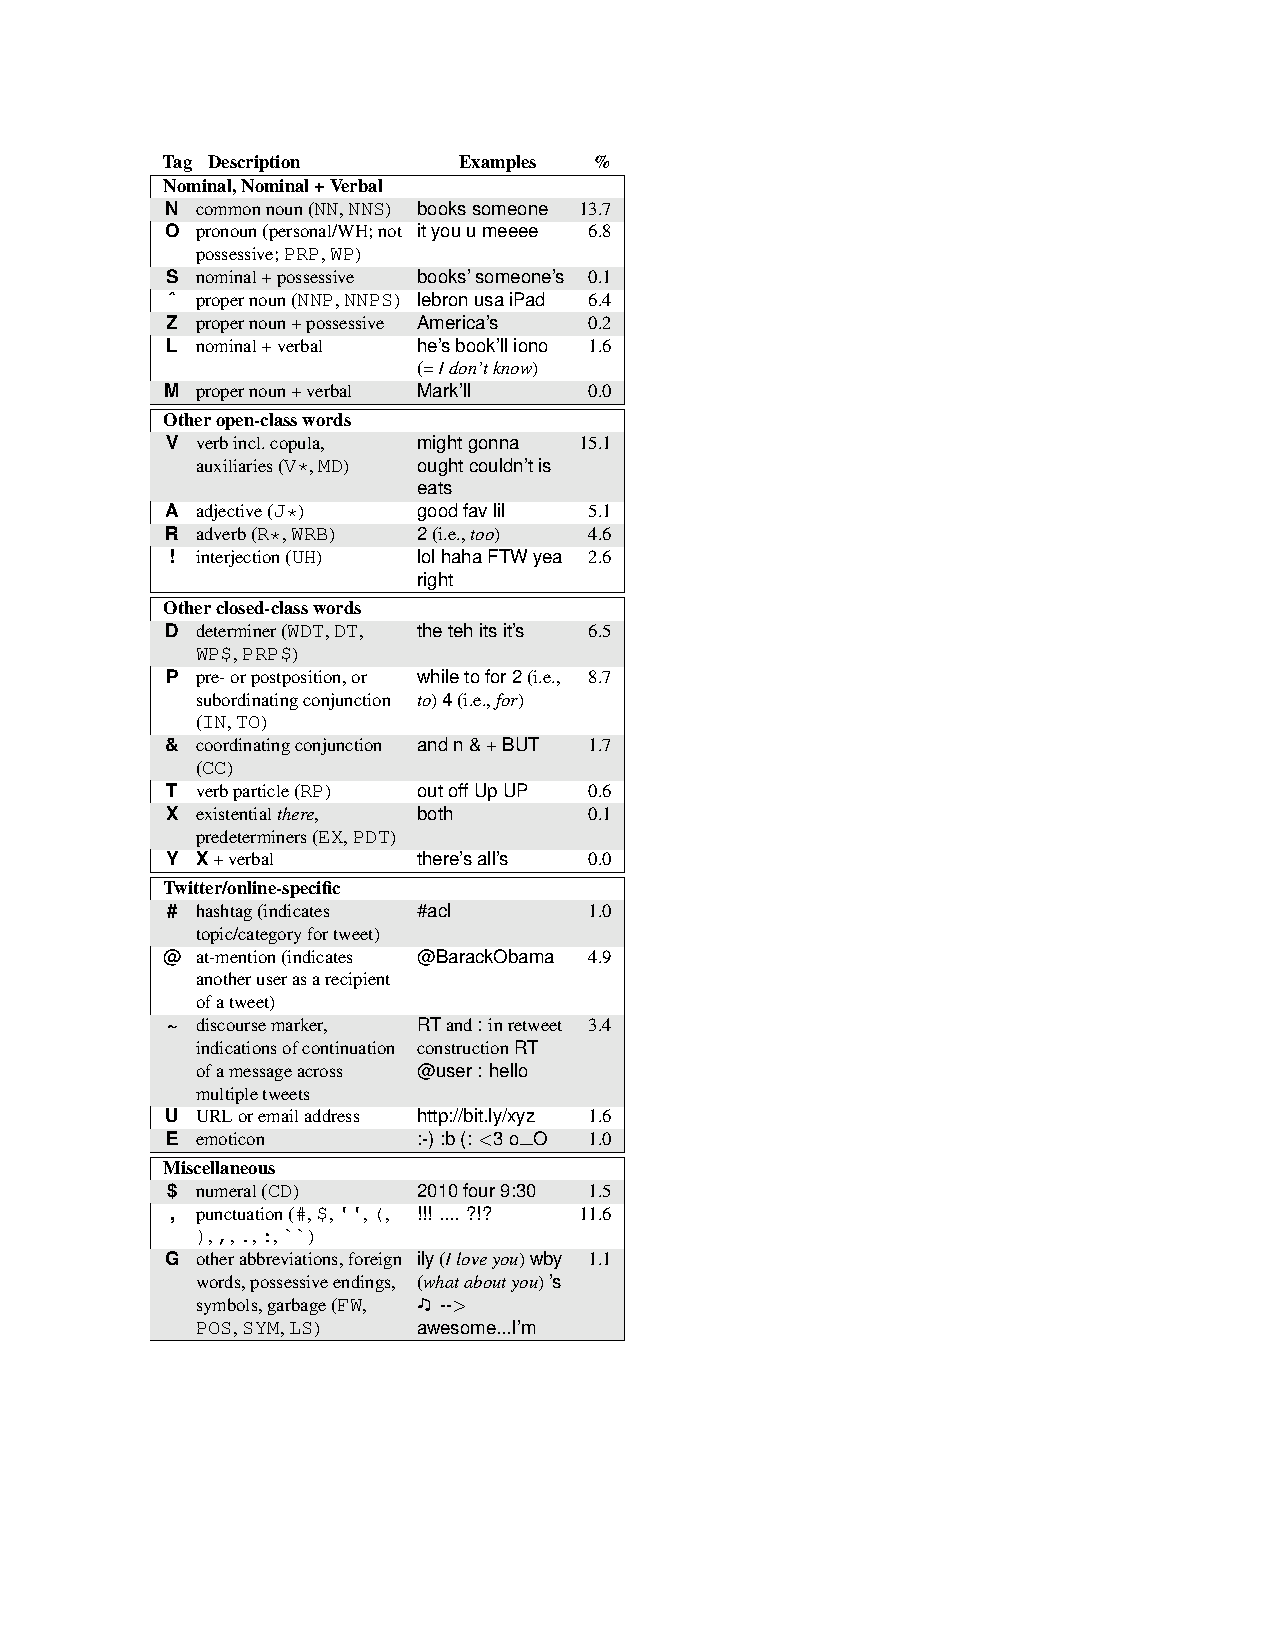
\includegraphics[width=.5\textwidth]{tags.pdf}
\caption{Tags as defined in source \cite{arkTagger}. Image taken from source.}
\label{fig:tags}
\end{figure}

\section{Results}
On initial testing with a training set of 999 sentences, and over 10 iterations, the model predicted a development set of $326$ sentences with $78.07\%$ correctness. To further analyze the robustness of this model, we break up the correct/incorrect tags in terms of whether or not a word being tagged has been seen before. Unsurprisingly, words that were not seen in training are tagged incorrectly with a higher percentage.
\begin{table}[h]
\begin{tabular}{ l | c }
& Percent\\
\hline
Correct Labels & 78.07\\
 Percent Correct Labeling of Unseen Words& 66.27\\
 Percent of Incorrectly Labelled Words Not Seen Before& 52.81 \\
\label{tab:unseenWords}
\end{tabular}
\caption{Percent correct labelings, and data on words not seen in training.}
\end{table}

In order to make improvements to this model, we want to analyze which parts of speech were being labelled incorrectly with the highest frequency. So we broke up this percentage up by label to determine given a part of speech, how frequently this word would be tagged incorrectly. In Figure 2 we see a bar graph of this percentage, compared to the tag frequency over the development data set. By examining this data, we can make a list of parts of speech that the model seems to handle particularly badly: \\

\begin{tabular}{ l | c }
Number of Times Tagged Wrong Higher than Mean & Tagged Wrong $50\%$ of the time\\
\hline
N Noun & S Possesives\\
\^{} Proper Noun & \^{} Proper noun\\
V Verb & Z Proper noun possessive \\
A Adjective & X Existential there\\
R Adverb & G Twitter abbreviations\\
G Twitter abbreviations &\\
\hline
\end{tabular}
\\

We see that the words in the left column tend to be parts of speech that simply occur with very high frequency: such as nouns, verbs, and adjectives. This is what we expect, because for this column we just used the raw number of wrong labelings, broken up by part of speech. And the words in the left column tend to occur with very low frequency: such as existentials and possessive proper nouns. However, two labels appear in both tables: \^{} and G. This indicates that the types of words that the model handles the poorest are proper nouns and Twitter abbreviations and colloquialisms. This is not surprising: unlike in traditional texts, proper nouns in Twitter statuses are not systematically capitalized, and words that are not proper nouns are capitalized. The makes labeling proper nouns much more difficult. And Twitter abbreviations often do not have even a typical part of speech in English, as they can represent whole phrases.

\begin{figure}
\centering
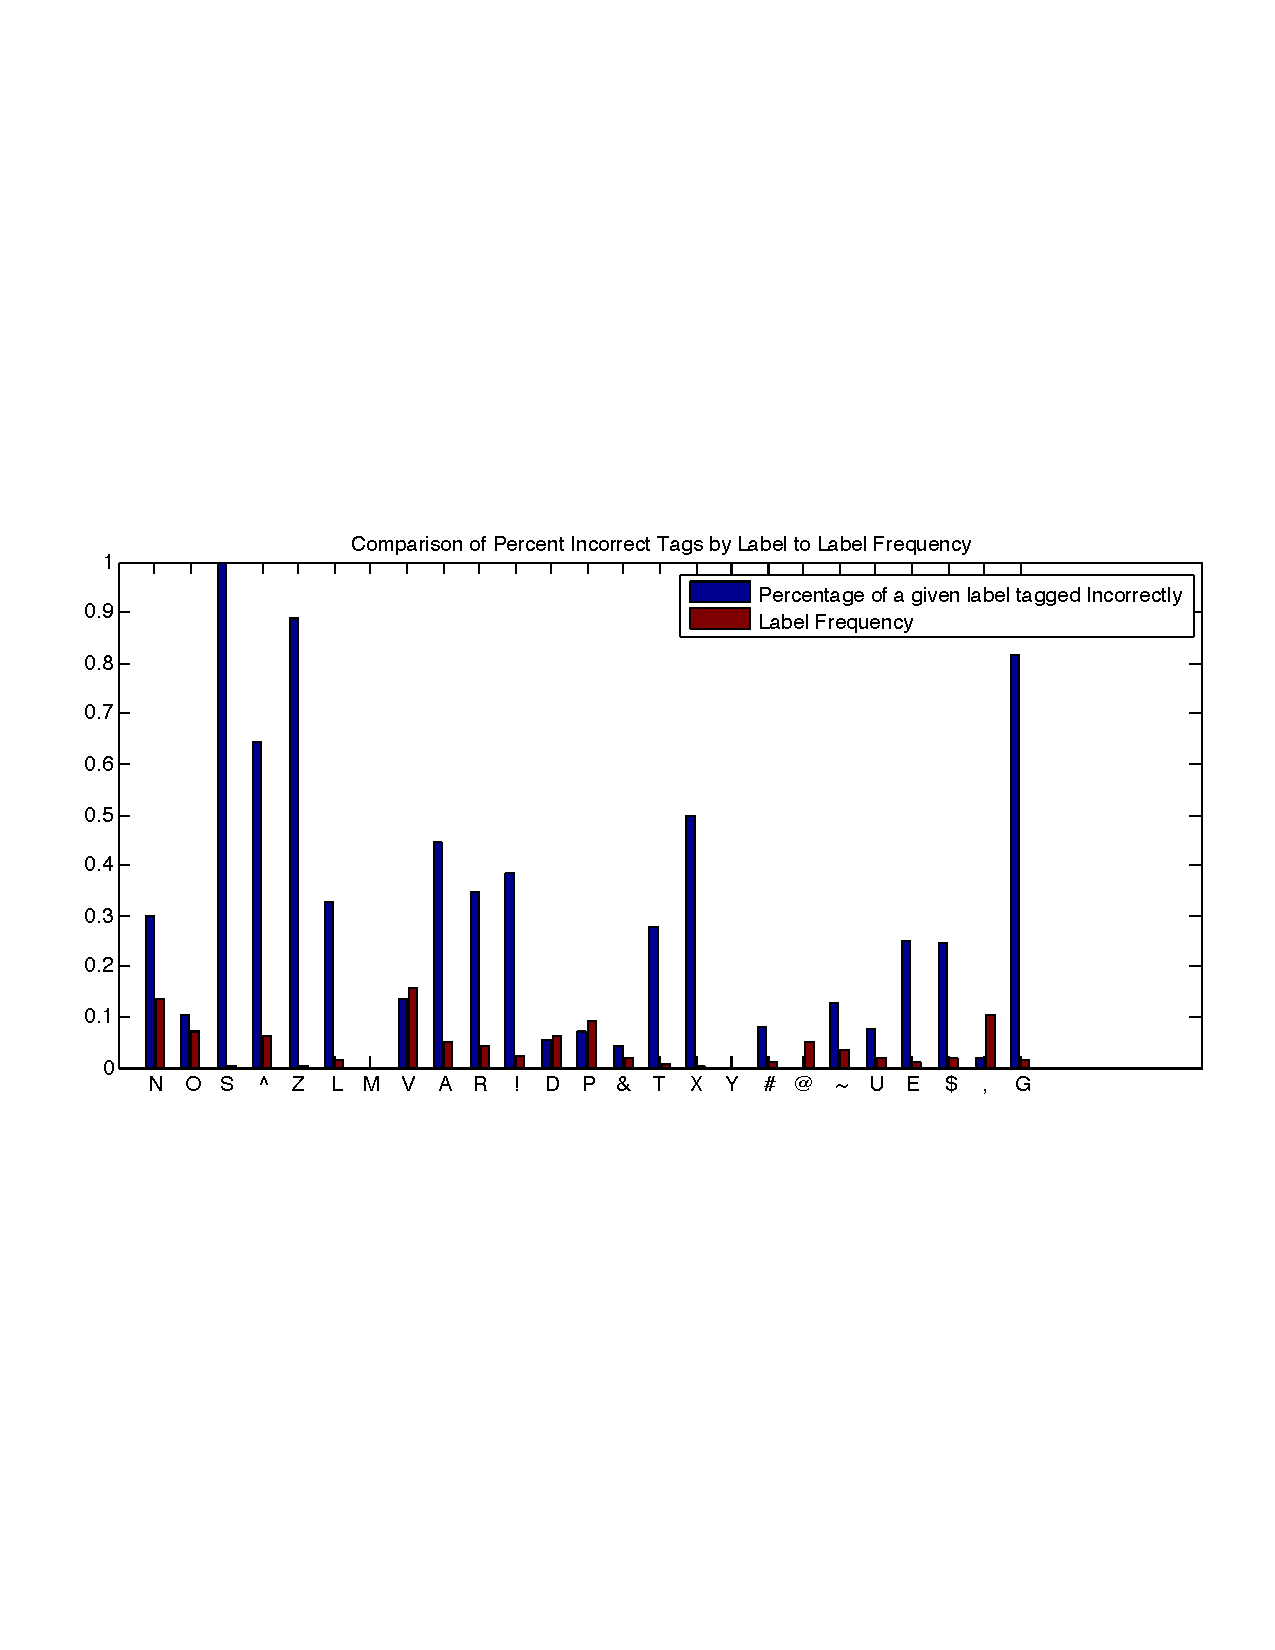
\includegraphics[width = .85 \textwidth]{comparison.pdf}
\label{fig:comparison}
\caption{A side-by-side comparison of the frequency of each label being tagged incorrectly, and that tag's frequency in the dev. data set.}
\end{figure}

\section{Improvement on Initial Results}
There are a couple clear areas for improvement from this simple model.
\begin{enumerate}
 \item The first is improving the tagging of proper nouns and Twitter slang and abbreviations. In order to improve the model's tagging of proper nouns and colloquialisms, we create a tagging dictionary. This tagging contains words and preassigned labels, and in the predict algorithm, before predicting a label, the model first checks to see if the word is in the tagging dictionary. If so, the model skips the predict step and automatically labels the word with the part of speech in the dictionary. The dictionary contains common names, cities, and corporations, labeled as proper nouns. The dictionary also contains a list of common colloquialisms, labelled as a Twitter expression. In addition, I experimented with adding words in the training set that had a given label $90\%$ of the time or more to the tagging dictionary, but this did not improve results.
 
\item Next I improved the tagging of unknown words, since this results in $50\%$ of the incorrect tagging decisions. The simplest way to approach this problem is to increase the training data size. The training sample was increased by training on an additional $547$ tweets as well as the original $1,000$ tweets. When we did so, we found that the percent correctness increased by $2.1 \%$ to $82.2\%$.
\end{enumerate}

%For this, we used the data in \cite{gateTagger}. Though this data was tagged with a different tag system, this tagging system was more specific than the one used in Gimpel et. al, making it possible to translate into the tagging system used here in this paper. However, I found that training on this data did not improve the accuracy of the model. The reason of this could be that the two tagging systems do not, in fact have the correct correspondence.

\section{Final Results and Comparisons}
Below is how this model compares to the ArkTagger from \cite{arkTagger}, trained on their annotated training data. Included for comparison is the Stanford tagger, which has also been trained on Twitter data from Gimpel et al.
\\

\begin{tabular}{ c  c c}
\hline
& \bf{Dev. Data} & \bf{Test Data}\\
\hline
ArkTagger &88.67 &89.37\\
Stanford Tagger &85.56 &85.85\\
Deirdre Tagger &80.05 &79.38
\end{tabular}
\\
\\

Additionally, in order to compare the model here to Derczynski, et. al, I adjust the model to handle Dercynski's much more fine-grained POS-labels (49 total labels rather than the Ark-dataset's 25 labels). Derczynski, et al. comprehensively compare the performance of their tagger with state-of-the art taggers, and break down correctness into percent-sentence correctness and percent-token correctness (in English, a token almost always means a word). For this reason I thought it was important to be able to compare this tagger with the tagger from Derczynski, et. al. Here I use the training, development and testing datasets provided in this paper. We find that the model performs better on the Ark tagger labelled data. This is expected, as there are many fewer tags in the Ark tagger label set. Additionally, the slang dictionary could not be used for comparison with the tagger from Derczynski, et al., as there was not one tag for Twitter abbreviations in this tagging system.\\
\\

\begin{tabular}{llrll}
\hline
 \bf{Tagger}& \multicolumn{2}{c}{\bf{Dev.}} & \multicolumn{2}{c}{\bf{Test}}\\
  & \bf{Token} & \bf{Sentence} & \bf{Token} & \bf{Sentence}\\
\hline
T-Pos Tagger (Ritter et al. 2011)  &  84.83 & 28.00 & 84.55 &  9.32\\
Derczynski, et al.  & 89.37 & 36.80 & 88.69&  20.34\\
Stanford Tagger & 83.14 & 6.78 & 84.19 & 24.07\\
Deirdre Tagger & 74.11 & 14.52 &75.03&13.33\\
\end{tabular}
\\
\\
\begin{figure}
\centering
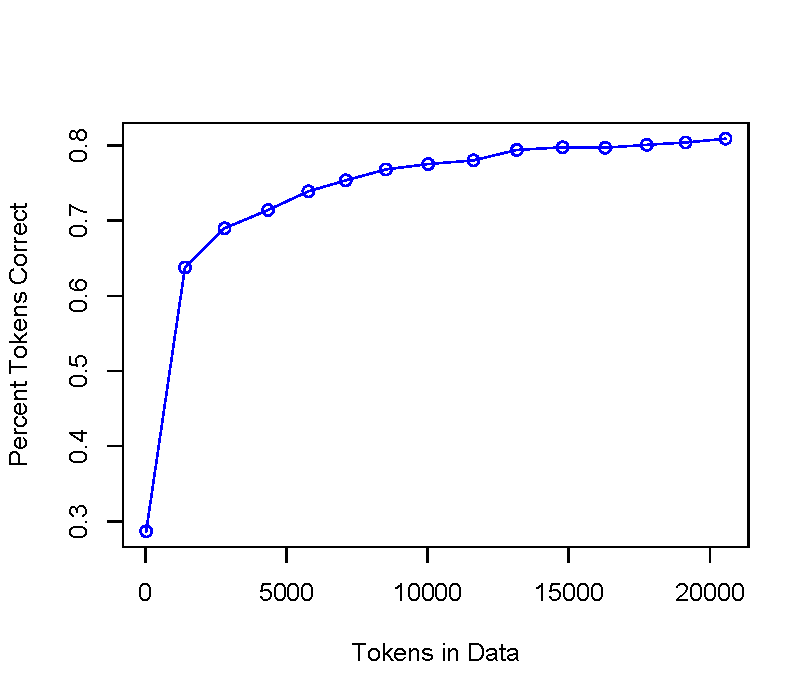
\includegraphics[width=.6 \textwidth]{tokens}
\label{fig:tokens}
\caption{The percent of correct labelled tokens when the data set is gradually increased.}
\end{figure}

\begin{figure}
\centering
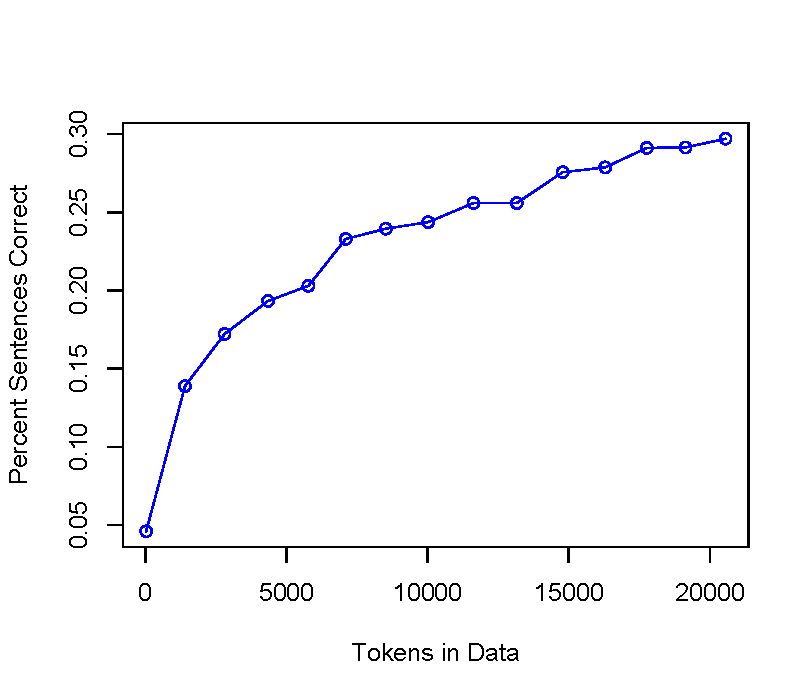
\includegraphics[width=.6 \textwidth]{sentTokens}
\label{fig:sentences}
\caption{The percent of entire sentences that are labelled corrected when the data set is gradually increased.}
\end{figure}

In Figures 3 and 4, we plot the percent of correct labeling of tags and whole sentences respectively, when the data size is increased. Note that the percent of sentences fully corrected tagged increases more steeply with the size of the data set. Finally, we compare the performance of the basic model to its performance with a tagging dictionary for slang words and proper nouns. We perform this test on the Ark test data set.
\\

\begin{tabular}{ c  c c}
\hline
\bf{Model} & \bf{Tokens} & \bf{Sentences}\\
\hline
Initial Model &78.07 & 26.88\\
Model with tagging dictionary &80.05 &27.50\\

\end{tabular}
\\
\\

In conclusion, we designed a Twitter POS-tagger using the averaged perceptron technique, which as far as I know has not yet been used for Twitter POS-tagging. This incredibly simple model performed not much worse than the Stanford tagger, a tagger that is state-of-the-art for POS-tagging of traditional texts. For whole sentences correctly, this tagger sometimes did better than the Stanford and T-POS tagger. Additionally, the performance of this tagger was only $8.67\%$ worse than the Ark Tagger, though its performance on the more refined tagset was not as good. Given the simplicity of this model (less than 400 lines of code) in comparison to considerably more models, a complex conditional random field model (the ark tagger), and a maximum entropy dependency network (Stanford tagger), I think that the averaged perceptron is a very effective tool for Twitter part of speech tagging. 

Some notable extensions that I would want to make for this model are the following:
\begin{enumerate}
 \item The addition of twice as many features, representing more features of the surrounding words in the sentence, as in \cite{bootstrap}. 
\item Another interesting extension would be to adapt this model to train on partially supervised data rather than fully supervised data, a technique called ``bootstrapping," used in \cite{gateTagger} and \cite{bootstrap}. I regret that I did not have time to implement this technique for this project, as I think the results would be very interesting. A ``bootstrapping" method would make sense for the problem of Twitter POS-tagging in particular, as the available labelled data is significantly smaller than that used for POS-tagging of traditional texts (for example, the standard Wall Street Journal data set includes one million words).
\end{enumerate}

\section{Appendix}

\verbatiminput{initAndRun.m}

\subsection{Features}
\verbatiminput{get_features.m}

\subsection{Prediction Algorithm}
\verbatiminput{predict.m}

\subsection{Updating Weights}
\verbatiminput{update.m}

\subsection{Training Algorithm}
\verbatiminput{train.m}

\subsection{Testing}
\verbatiminput{testAlg.m}

\begin{thebibliography}{9}
\bibitem{wikiPOS} ``POS Tagging (State of the Art)." - ACLWiki. Wikipedia, 5 May 2013. Web. 12 Dec. 2013.

\bibitem{collins} Collins, Michael. 2002. Discriminative Training Meth- ods for Hidden Markov Models: Theory and Exper- iments with Perceptron Algorithms. In EMNLP �02: Proceedings of the ACL-02 conference on Empirical methods in natural language processing, volume 10, pages 1�8, Philadelphia, PA.

\bibitem{perceptron} Dame, Hall, III. "The Perceptron." A Course in Machine Learning. N.p., n.d. Web.

\bibitem{arkTagger} Gimpel, K., Schneider, N., O'Connor, B., Das, D., Mills, D., Eisenstein, J., Heilman, M., Yogatama, D., Flanigan, J. \& Smith, N. A. (2011). Part-of-speech tagging for Twitter: annotation, features, and experiments. Proceedings of the 49th Annual Meeting of the Association for Computational Linguistics: Human Language Technologies: short papers - Volume 2 (p./pp. 42--47), Stroudsburg, PA, USA: Association for Computational Linguistics. ISBN: 978-1-932432-88-6

\bibitem{200words} Honnibal, Matthew. "Computational Linguistics." Computational Linguistics. N.p., Sept.-Oct. 2013. Web. 12 Dec. 2013.

\bibitem{sentiment} Kouloumpis, E., Wilson, T., \& Moore, J. (2011, May). Twitter sentiment analysis: The Good the Bad and the OMG!. In ICWSM.

\bibitem{twitterBlog}Krikkorian, Raffi. "New Tweets per Second Record, and How! | Twitter Blogs." Twitter Blogs. Twitter, Inc., 16 Aug. 2013. Web. 12 Dec. 2013.

\bibitem{gateTagger}L. Derczynski, A. Ritter, S. Clarke, and K. Bontcheva. 2013. "Twitter Part-of-Speech Tagging for All: Overcoming Sparse and Noisy Data". In Proceedings of the International Conference on Recent Advances in Natural Language Processing, ACL.

\bibitem{bootstrap} Spoustov\'{a}, Drahom\'{\i}ra "johanka" and Haji\v{c}, Jan and Raab, Jan and Spousta, Miroslav. 2009. Semi-supervised training for the averaged perceptron POS tagger. In Proceedings of the 12th Conference of the European Chapter of the Association for Computational Linguistics (EACL '09). Association for Computational Linguistics, Stroudsburg, PA, USA, 763-771.

\end{thebibliography}


\end{document}  